\chapter{Theoretical background}
\section{Computer vision tasks}
\begin{figure}
    \centering
    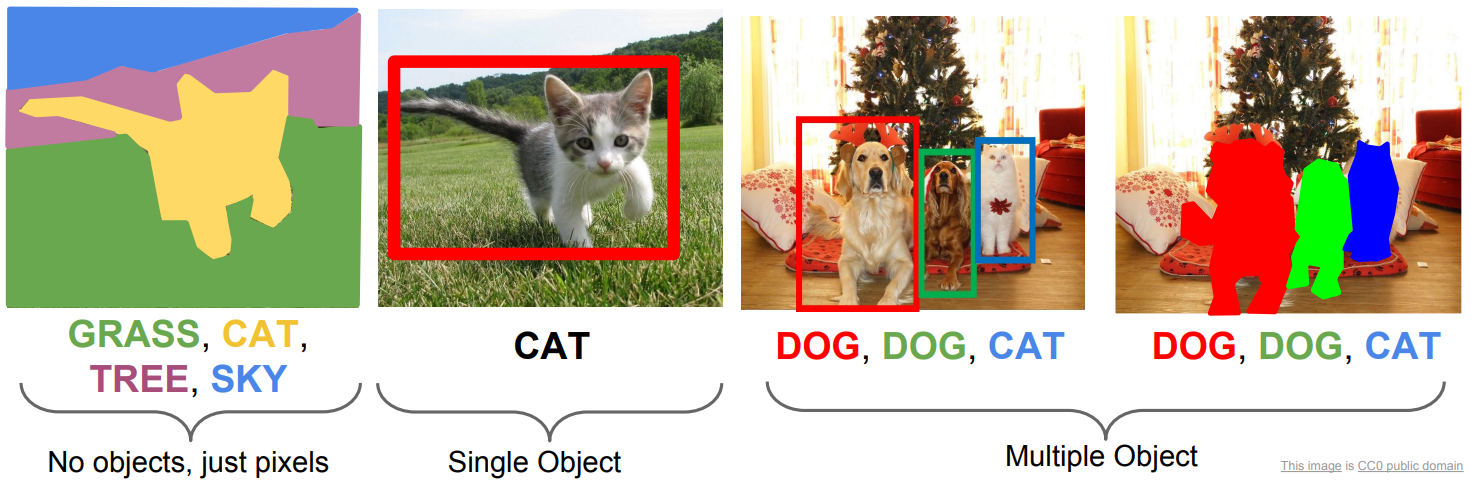
\includegraphics[width=\linewidth]{images/computer_vision_tasks.png}
    \caption{From the left: semantic segmentation, object localization, object detection, instance segmentation}.
    \label{fig:computer_vision_tasks}
\end{figure}
This section provides a quick overview of standard computer vision tasks.
\subsection{Classification}
Let's say we have an image $\mathbf{x}$. In a classification task, our goal is to assign one of $n$ possible classes to the image:
\begin{align}
    \hat{y} = f_\theta\left(\mathbf{x} \right),
\end{align}
where $f$ is a mapping, sometimes called a model, and $\theta$  represents model parameters. If it holds that $\hat{y}=y$, where $y$ is a true class of the image $\mathbf{x}$, the classification is considered to be correct.
It is possible to output $\mathbf{p} \in \mathbb{R}^n$ instead of $\hat{y}$, where $p_i \in \mathbf{p}$ is probability of $i = y$, modeled by $f_\theta$.

\subsection{Semantic segmentation}
For an input image $x \in \mathbb{R}^{n \times m}$ the goal is to output $\mathbf{\hat{Y}} \in \mathbb{R}^{n \times m}$, where $y{_i,j}$ is predicted class of pixel $i,j$ in the image $\mathbf{x}$. Similarly to classificaiton problem we can output matrix $\mathbf{P} \in \mathbb{R}^{n \times m \times c}$, where $p_{i,j,c}$ is probability of $pixel_{i,j}$ belonging to class $c$. A sample of semantic segmentation output can be seen in figure \ref{fig:computer_vision_tasks}.

\subsection{Object detection}
\label{subsec:object_detection}
In object detection, the goal is to locate and recognize objects of interest in the image $\mathbf{x}$. A ground truth object is represneted by a rectangle and a category. Model predicts $\mathbf{Y} \in \mathbb{R}^{n \times 6}$ values for each image. Each row of $\mathbf{Y}$ consists of four numbers, which describe a rectangle, the category of the object inside the rectangle, and a number in the range from 0 to 1 called the confidence. In literature, we can see term score instead of confidence, but the meaning remains the same: Certainty of the network regarding the particular prediction described by the bounding box and category. Please note that the confidence of predictions does not sum to one; in other words, we are not talking about probabilities since multiple detections per image can correspond to ground truth.

\subsection{Instance segmentation}
Instance segmentation is similar task to semantic segmantation with the difference, that two objects of the same category would have different ground truth values. If we have $\mathcal{O}_1, \mathcal{O}_2$, where $\mathcal{O}_i \subset \mathbf{x}$ are pixels of object $i$ in image $\mathbf{x}$. Then
\begin{align}
    o_{1_i} \neq o_{2_i} \quad \text{for} \quad o_{1_i} \in \mathcal{O}_1, o_{2_i} \in \mathcal{O}_2;\forall i
\end{align}

\section{Data format in object detection}
As described in section \ref{subsec:object_detection}, the position of an object is denoted by a bounding box.  The four parameters used to describe a bounding box can be selected in multiple ways. This ambiguity led to disjoint notation. The most widespread are as follows.
\subsection{PASCAL VOC}
The format was introduced together with the PASCAL VOC dataset, which was the most popular dataset for object detection algorithm benchmarking in 2010. The bounding box is described by points $p_1(x,y),p_2(x,y)$ located in the top-left and bottom right corner. The coordinates range from 0 to image width/height in pixels. All the annotations are stored into single XML file \cite{Everingham2009,Padilla2021}.
\subsection{COCO}
COCO data format is represented by a single JSON file containing all bounding boxes of the dataset. The boxes are described by the top-left corner point $p(x,y)$ and the width and height of the box. Coordinated and box dimensions are again in the range 0 to image dimensions. In MS COCO, the annotation can be accompanied by additional information to solve the task as an instance segmentation problem.
\subsection{YOLO}
This format was introduced together with the first YOLO architecture \cite{Redmon2015}, and this annotation style is still persistent whenever working with the YOLO-family neural networks.
The annotations are divided into multiple TXT files in this format. Each of them contains annotations for a single image.
The bounding box is described similarly to the COCO dataset, but the coordinates are normalized to be in the 0 to 1 range. The advantage of this approach is that when image dimensions are scaled, the annotations do not have to be modified \cite{Redmon2015, Padilla2021}.


\section{Metrics}
\subsection{Intersection over union (IOU) }
Intersection over union, also known as Jaccard index, is defined as follows: Let $B_{gt}$ and $B_p$ be a ground truth and predicted bounding box, and the Jaccard index $J$ is calculated as
\begin{align}
    IOU = J(B_p, B_{gt}) = \frac{area(B_p \bigcap B_{gt})}{area(B_p \bigcup B_{gt})}.
    \label{eq:iou}
\end{align}
From the equation \ref{eq:iou} we can see that the the lowest value of IOU is 0. That means there is no overlap at all and the maximal value is 1, hence meaning a perfect match.
We use predefined threshold value of IOU to decide if the predicted bounding box matches the ground truth. Usually we choose this threshold to be 0.5 or above.

IOU can be defined for semantic segmentation task with two classes (eg. background and target class). Let $\mathbb{\hat{Y}} \in \mathbb{R}^{m \times n}$ be a mask of predicted values, where $\hat{y}_{i,j} = 1$ if the model predicts, that pixel $i,j$ belongs to target class. The IOU is defined as:
\begin{align}
    IOU = \frac{\sum_{i=1}^{m} \sum_{j=1}^{n} \hat{y}_{i,j} \wedge  y_{i,j}}{\sum_{i=1}^{m} \sum_{j=1}^{n} \hat{y}_{i,j} \vee  y_{i,j}}
\end{align}
where $y_{i,j} \in \mathbf{Y} \in \mathbb{R} ^ {m \ times n}$ is ground truth value for pixel $i,j$.


\begin{figure}
    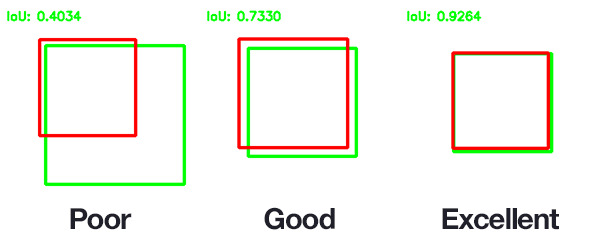
\includegraphics[width = \linewidth]{images/IOU.jpg}
    \caption{Examples of IOUs for different overlaps between GT and predicted box, source \cite{Cowton2019}}
    \label{fig:iou}
\end{figure}

\subsection{Precision and recall}
\subsubsection{Precision}
\label{subsec:precision}
When speaking about object detection, we say that a prediction is a true positive (TP) if the IOU value is greater than the predefined threshold $\tau$. If otherwise, the prediction is treated as a false positive (FP). Let's assume there are N predictions of our model, from which S are correct. Precision is defined as
\begin{align}
    Precision(\tau, \gamma) = \frac{TP(\tau, \gamma)}{TP(\tau, \gamma) + FP(\tau, \gamma)}
\end{align}
where $\gamma$ is confidence threshold. That means we discard all predictions with confidence smaller than $\gamma$. Note that for fixed value of $\tau$ are $FP(\gamma)$ and $TP(\gamma)$ decreasing functions of $\gamma$ \cite{Padilla2021}.

\

\subsubsection{Recall}
\label{subsec:recall}
If there is a ground truth bounding box for which there are no given detection values of $\gamma$ and $\tau$, we say it is a false negative (FN). If we consider a dataset with G ground-truths and N predictions of which S is correct, where $(S \leq G)$, the recall is expressed as:
\begin{align}
    Recall(\tau, \gamma) = \frac{TP(\tau, \gamma)}{ TP(\tau, \gamma) + FN(\tau, \gamma)}.
\end{align}
Since the value of $FN(\gamma)$ increases with the growing value of $\gamma$, we see that recall is the decreasing function of $\gamma$.

\subsubsection{F1 score}
The value of the F1 score is computed as the harmonic mean of precision and recall.
\begin{align}
    F1(\tau, \gamma) = \frac{2 \cdot Recall(\tau,\gamma) \cdot Precision(\tau, \gamma)}{Recall(\tau,\gamma) + Precision(\tau, \gamma)}
\end{align}

\subsubsection{Precision-recall curve}
From subsection \ref{subsec:precision} and \ref{subsec:recall} we were able to see that precision mostly increases as we increase the confidence threshold $\gamma$, while recall decreases. The relation between precision and recall is captured by precision-recall curve. An example of precision-recall curve can be seen as the blue line in the figure \ref{fig:pr_curve}. In other words, we can say that the precision-recall curve is a mapping
\begin{align}
    \gamma \rightarrow Precision(\gamma) \times  Recall(\gamma),
    \label{eq:pr_curve}
\end{align}
where $\gamma$ ranges from 1 to 0.

\subsubsection{Mean average precision (mAP)}
To calculate MAP we first need to get the PR-curve and then interpolate the precision values. Suppose, that we have $K$ different confidence values $\gamma$ among model predictions, which are ordered as
\begin{align}
    \gamma(k),\: k = 1,2,...,K,  \; \text{such that } \gamma(i) > \gamma(j) \: for \: i > j.
\end{align}
The interpolated precision-recall curve is defined as
\begin{align}
    Precision_{interp}(R) = \max_{k|Recall(\gamma(k)) \geq R} \{  Precision(\gamma(k)) \},
\end{align}
where $R$ is a real value contained in interval [0,1] \cite{Padilla2021}.
The interpolated precision-recall is pictured in the figure \ref{fig:pr_curve} in red color. Now, we can compute the average precision (AP) as the area under the interpolated PR curve.
In practice, there are two different ways to approach the Reimann integral. They differ in the number of samples used to compute the integral and are called N-point and all-point interpolation. The N-point, specifically 101 point interpolation, is used in the MS COCO competition. On the other hand, the all-point interpolation is nowadays used in PASCAL VOC challenges \cite{Padilla2020, Padilla2020}.

Since the AP is calculated per class, the mean average precision is defined as the average over all categories.

In the subsections, \ref{subsec:precision} and \ref{subsec:recall}, we said that both precision and recall depending on predefined IOU threshold $\tau$ to consider prediction as true positive. This dependency makes the value of MAP vary over different values of $\tau$. The threshold value used for computation of the mAP is usually denoted in the metrics name, such as $AP@.5$ in the case of MS COCO. \footnote{Note that even though the mean average precision is computed, the $AP$ shortcut, which stands for average precision, is used.} The standalone $AP$ without any numerical values attached to it usually refers to the official COCO metric. The official COCO metric is in its explicit form written as $AP@[.5:0.05:0.95]$ and is computed as the average of MAP values for ten different $\tau$ values, ranging from 0.5 to 0.95.

The letters S, M,  and L in the subscript, such as $AP_S$ denote that the metrics are calculated for a subset of ground truth predictions only. Taking into the consideration only bounding boxes with area $\leq 32^2$ pixels, $32^2 \le $ area $ \leq 96^2$ pixels and area $> 96^2$ pixels

\subsection{Mean avarage recall (mAR)}
MS COCO uses little bit different definition of recall, than the one described in section \ref{subsec:recall}. In the MS COCO case, they sort predictions in descending order by their confidence score and take only top $n$ of those. After that, they callculate how many ground TODO finish this

TODO


\begin{figure}
    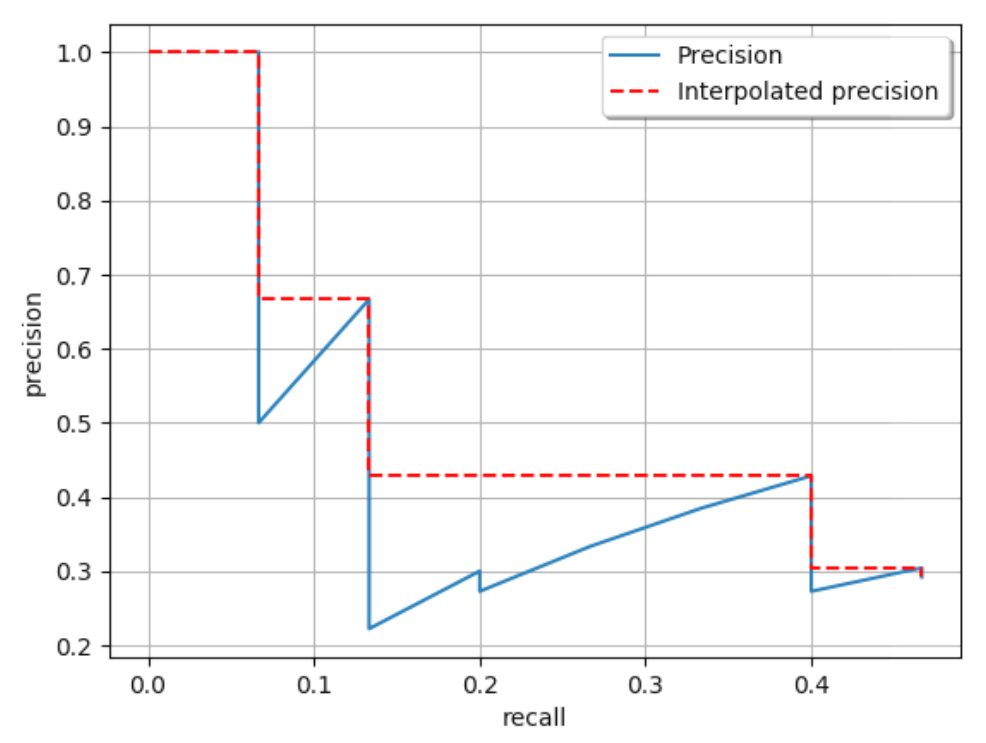
\includegraphics[width = \linewidth]{images/PR-curve.png}
    \caption{Normal and interpolated precision-recall curve, source \cite{Padilla2020}}
    \label{fig:pr_curve}
\end{figure}


\subsubsection{Dice Loss}
TODO

\subsubsection{Cross-Entropy loss}
TODO


\section{Optimization}
\subsection{Optimizers}
\subsubsection{Adam}
TODO
\subsubsection{AdamW}
TODO
THIS SECTION IS UNFINISHED

\subsection{Learning rate schedulers}
TODO rewrite Learning rate is considered to be one of the most, if not the most important parameter, in deep learning. It is usually beneficial to change the learning rate during the course of training. This can be done either manually or can be automated by an algorithm that increases or decreases the learning rate based on the set of predefined rules. This algorithm is called learning rate scheduler.

\subsubsection{Reduce learning-rate on plateau}
TODO rewrite We couple the scheduler with a model metric and when the improvement of the metric stalls for a predefined period of time, the learning rate is decreased.
The scheduler is not heavily reliant on the setting of it's hyper-parameters, making it for most of the developers a go-to choice to start from.
\subsubsection{Cosine }
TODO

\subsection{Image augmentations}
TODO


\section{Arificial neural network (ANN)}
Arificial neural networks are inspired by the mechanisms of human brain. Human neuron cells are in ANN replaced replaced by artificial neurons, which are difined as:
\begin{align}
    y = f \left( \boldsymbol{w}^T \boldsymbol{x}  + b \right).
\end{align}
Where $\boldsymbol{x}$ is vector of inptus, $\boldsymbol{w}$ are weights and $b$ is bias. Symbol $f$ denotes an activation funtion f : $\mathbb{R} \rightarrow \mathbb{R}$. The artificial neuron proposed by Frank Rosenblatt in the perceptron algorithm used step funtion \cite{Rosenblatt1958}, but nowadays, different functions such as ReLu, sigmoid or tanh are used. The output of the neuron $y$ is called activation of the neuron.

Neurons are ussally structured into layers. The connection between layers is depended upon the architectural choice. First ANNs used fully connected layers, meaning that the input into a neuron in layer $n$ were composed of all activations from layer $n-1$. Fully connected neural networks are nowadays sparsely used in computer vision. Convolutional neural networks (CNNs) or vision transformers are used instead. In the case of CNNs we limit neurons' receptive field to the local neighborhood only; this decreases the computation complexity and includes our prior knowledge of pixel neighborhood in the input image. Having the same weights for the whole input makes the network invariant to shifts in the input.

\subsection{Convolutional layer}
Convolutional layers consists of $C_{out}$ neurons, each having $C_{in}, H, W$ receptive field. Those neurons are called kernels with width $W$ height $H$ and a number of input channels $C_{in}$. In each layer, we convolve\footnote{Even though we usually refer to convolution, in practice cross-correlation is used instead and terms cross-correlation and convolution are used interchangeably.} the input $X$  with the kernel $W$, the output $Y$ is defined by:
\begin{align}
    y_{o,i,j} = \sum_{c_{in}} \sum_{\Delta i} \sum_{\Delta j} x_{c, i+\Delta i, j + \Delta j}  w_{o,c, \Delta i, \Delta j}
\end{align}
Nowadays, modifications of convolutional layers are proposed, such as dilated convolution, grouped convolution, or depth-wise separable convolutions are used, but the fundamentals are the same: Filter sliding over the input produces an output.

\begin{figure}
    \centering
    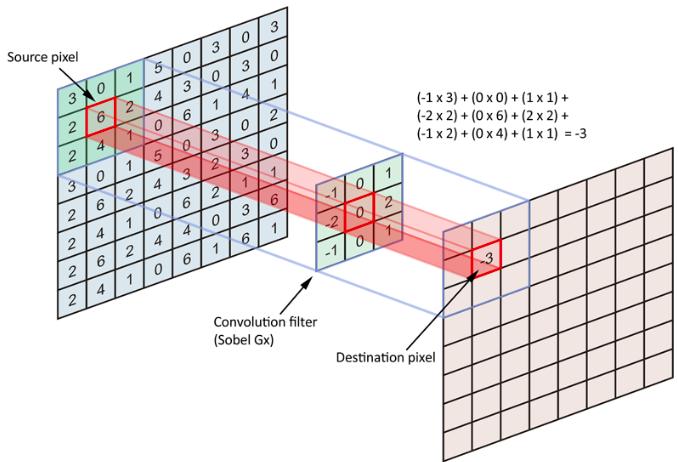
\includegraphics[width=0.9\linewidth]{images/conv_img.png}
\end{figure}

\subsection{Activation functions}
A non-linear activation function usually follows the output of the convolutional layer. Many activation functions are at our disposal, but the most commonly used is ReLU and its derivatives, such as SERLU, SELU, ELU, Swish, and Leaky ReLU. Values of those function are depicted in figure \ref{fig:activation_functions}.

\subsection{Normalization layers}
\subsubsection{Batch-normalization}
TODO
\subsubsection{Group-normalization}
TODO

\begin{figure}
    \centering
    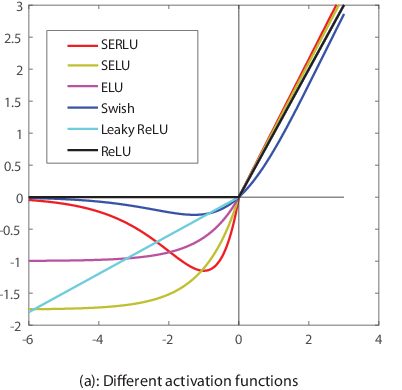
\includegraphics[width=0.6\linewidth]{images/activation_functions.png}
    \caption{Graphs of ReLU based activation functions, source \cite{Zhang2018}}
    \label{fig:activation_functions}
\end{figure}


\section{Transformer architecture}
Transformer architecture debuted in computer vision in 2021 and since then achieved outstanding results, beating state-of-the-art models in multiple benchmarks across all computer vision tasks. As of May 2022, the best-performing models in the main computer vision benchmarks are based on transformer architecture. We think of the following benchmarks to be the main ones in computer vision:  ImageNet benchmark (classification task), COCO (object detection), ADE20K (semantic segmentation).

The transformer architecture was proposed already in 2017 for the task of natural language processing (NLP); we will briefly introduce transformer architecture for the NLP task since it is crucial for the understanding of transformers for computer vision.

\subsubsection{Transformers in NLP}
Transformer architecture was introduced in the paper Attention is all you need \cite{Vaswani2017} for NLP. NLP is a task where input is a sequence of words of length $n$ and output is a sequence of $m$ words, where $n$ and $m$ usually differ. The sequence of words is converted into a sequence of vectors. There are multiple options for how to embed words into vector, commonly used is TD-IDF or Word2Vec\cite{Li2018}. Positional encoding is added to those vectors are then processed by the encoder block. The novel key component is the self-attention module, where for the input sequence of vector values $V$, keys $K$ and queries $Q$ are computed. From encoder, we output values and keys, and from the decoder's self-attention module, we output queries. We then take keys and values from the encoder and queries from the decoder and input them into another attention block:
\begin{align}
    Attention \left(Q,K,V \right) = \text{softmax} \left( \frac{QK^T}{\sqrt{d_k}} \right)V,
\end{align}
where $d_k$ is dimension of keys. More details can be seen in figure \ref{fig:nlp_transformer} or in \cite{Vaswani2017}.

\begin{figure}
    \centering
    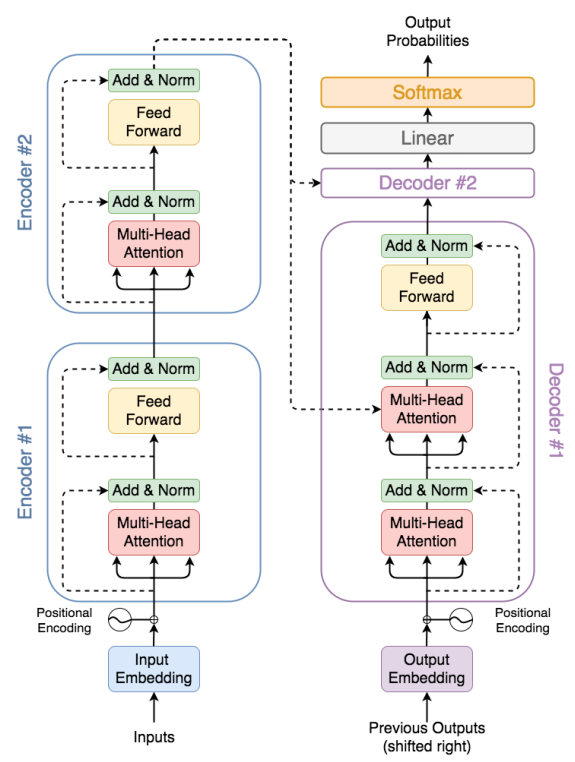
\includegraphics[width=\linewidth]{images/two_layer_transformer.png}
    \caption{Architecure of transformer with two encoders and two decoders, source \cite{Yin2020}}
    \label{fig:nlp_transformer}
\end{figure}

\subsection{Transformers in computer vision}
The first trasnformer-based model was Vision Transformer (ViT). It was capable of image classification only, and it is composed of multiple encoder blocks stacked on top of each other. Those blocks are the same as those used by the transformer for the NLP task. On the top encoder, blocks are attached multi-layer perceptron (MLP) head, which outputs values for each class. Those can be converted into corresponding probabilities by softmax-layer. Input into ViT are $16 \times 16$ image patches linearly projected into vectors; the whole architecture is shown in figure
\begin{figure}
    \centering
    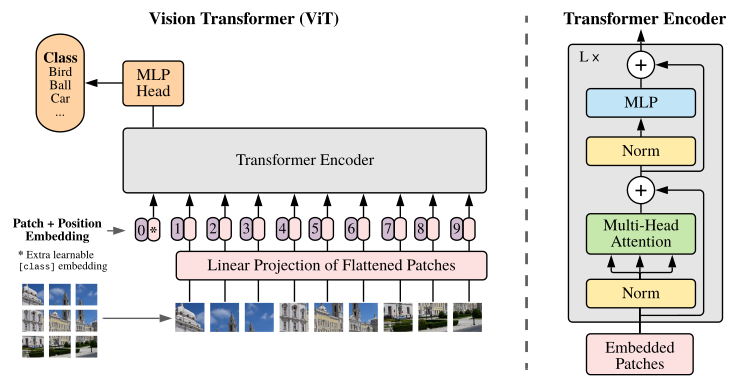
\includegraphics[width=\linewidth]{images/vision_transformer.png}
    \caption{Architecture of ViT, source \cite{Dosovitskiy2020}}
    \label{fig:vision_transformer}
\end{figure}


\section{General architecture for object detection}
Even though there is a wide variety of architectures for object detection, the core principles remain the same. The model is composed of three main parts: backbone, neck, and head, as shown in figure \ref{fig:object_detection_architecture}. Each of those blocks can usually be swapped for a different one, fulfilling the same purpose. This gives us great flexibility and allows us to try different combinations of those blocks.


\begin{figure}
    \centering
    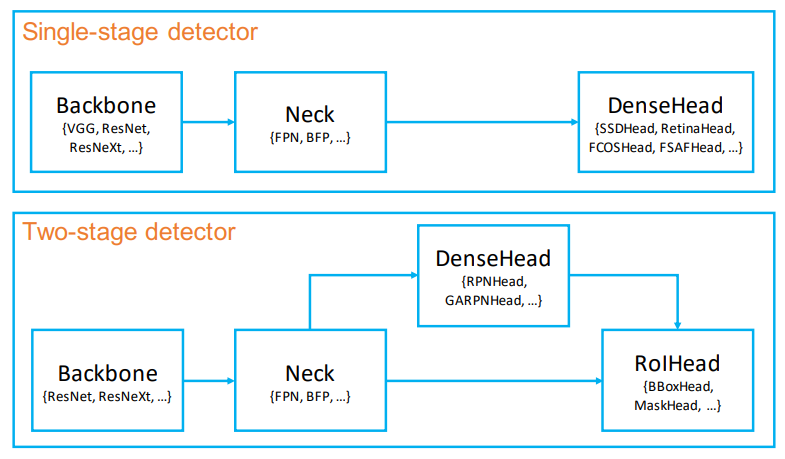
\includegraphics[width=0.6\linewidth]{images/object_detection_architecture.png}
    \caption{General architecture for object detection, source \cite{Chen2019}}
    \label{fig:object_detection_architecture}
\end{figure}

\subsubsection{Backbone}
The purpose of backbones is to transform the input image into feature maps. For this purpose, we use classification models with the classification head removed. Most parameters of object detection models are usually part of the backbone. Extraction of useful feature maps is vital for other blocks to perform well. The most common backbones are models from the ResNet family.

\subsubsection{Neck}
The neck is responsible for the merging of features from the backbone. This is not a straightforward task since we usually use features from different backbone layers. This allows us to get semanticaly strong features from deeper layers as well as more detailed information from earlier ones. Common neck architectures are feature pyramid network or PANet.
\begin{figure}
    \centering
    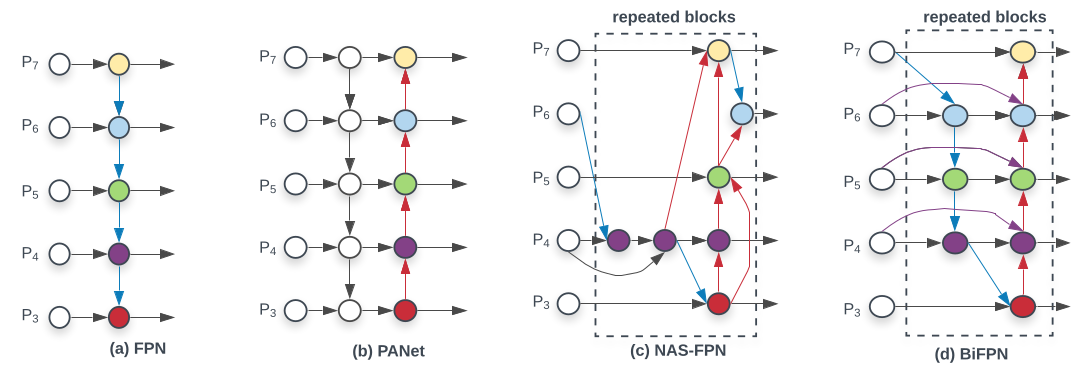
\includegraphics[width=\linewidth]{images/necks_architecture.png}
    \caption{Architecture of different necks for feature fusion, source \cite{Tan2019}}
    \label{fig:necks}
\end{figure}

\subsubsection{Head}

\section{Backbone models}
This section will introduce multiple architectures of neural networks, which were used as a backbone throughout our work.
\subsection{ResNet}
ResNet architecture was introduced by He et al. \cite{He2015} and proposed a novel element of deep-learning architectures - identity shortcut connection, sometimes called skip-connection. Let $\mathbf{x}$ be input into a block composed of multiple convolutional layers with activation functions in between\footnote{Addition of batch-normalization, or other layers is possible}; we will call this block a mapping $\mathcal{F}$. The output of residual block $\mathcal{H}$, derived from $\mathcal{F}$ is defined as:
\begin{align}
    \mathcal{H}\left(\mathbf{x}\right) = \mathcal{F} \left(\mathbf{x}\right) + \mathbf{x}.
\end{align}
The reasoning behind the residual block is to make it easier to learn identity mapping if desired. This had other benefits, especially the improvement of gradient flow during back-propagation, making it easier to optimize such blocks. This ease of optimization can be seen by inspecting the loss function landscape of a model with and without skip-connections, figure \ref{fig:resnet_loss}.
Final ResNet architecture is composed of multiple residual blocks stacked one after another; the models vary in the number of layers used; this is denoted in the name with a number such as ResNet50 or ResNet101.

\begin{figure}
    \centering
    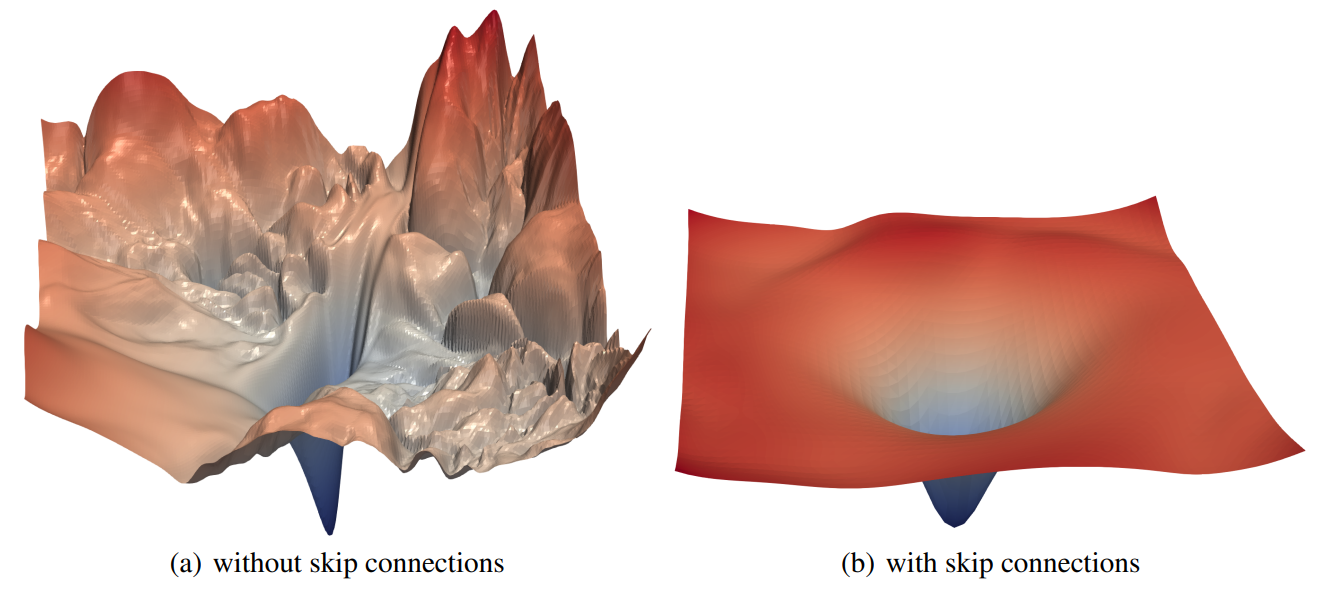
\includegraphics[width=\linewidth]{images/resnet_loss.png}
    \caption{Comparison of loss landscapes, source \cite{Li2017}}
    \label{fig:resnet_loss}
\end{figure}

\subsection{EfficientNet}
When scaling model size, we can increase: Number of layers (depth), the number of filters in each layer (width), or the width and height of feature maps (resolution). It has been common practice to change only one of them. Tan and Le \cite{Tan2019a} did a multi-objective neural network search, where they tried to maximize objective function $O$ defined as:
\begin{align}
    O = ACC \left( m \right) \times \left[ FLOPS \left(m \right) / T \right] ^w,
\end{align}
where $ACC(m)$ and $FLOPS(m)$ are accuracy and floating point operatoins (FLOPS) of model $m$, $T$ is target number of FLOPS and $w$ is a hyper-paremter controling the trade-off between accuracy and number of FLOPS of the final model. From this search resulted the EfficientNet-B0 baseline model, which can be scaled to obtain a bigger network, those are called B1-B7.

\subsection{Swin transformer}
Swin transformer architecture overcomes the limitations of ViT, which is working with $16 \times 16$ image patches only. This is insufficient for segmentation and object detection tasks, where dense predictions are needed. Swin transformers are in the first layer working with $4 \times 4$ patches. Since the computation complexity of the self-attention layer grows quadratically with a number of input tokens, the authors overcome this by using neighbor patches only. Attention is thus computed with respect to tokens in the non-overlapping local window. This local window for computing self-attention is shifted after every encoder layer, as depicted in figure \ref{fig:swin_pathces}. This shift introduces cross-window connections, which increases the modeling capacity of the model. After a particular number of encoder layers, neighbor patches are merged. This reduces the number of patches while increasing their size by a predefined factor. This mimics the behavior of CNNs, where we start with big, semantically weak feature maps and gradually decrease their dimensions while increasing their number. Having this kind of feature map allows using swin transformer as a general backbone for any task. \cite{Liu2021}

\begin{figure}
    \begin{floatrow}[2]
        \ffigbox[\FBwidth]{\caption{Hierachical structure of Swin Transformer compared with ViT, source \cite{Liu2021}}\label{fig:swin_hierarchy}}%
        {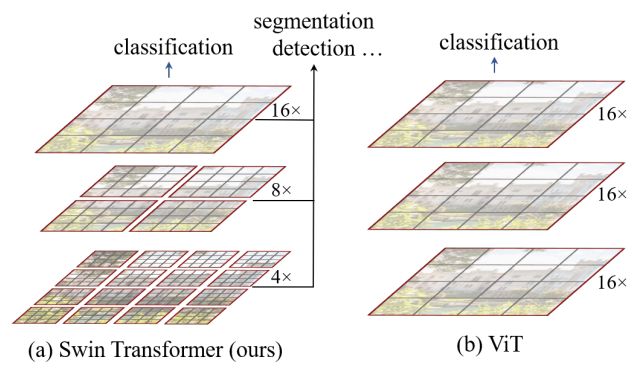
\includegraphics[width=\linewidth]{images/swint_transformer_hierarchy.png}}\qquad
        \ffigbox[\FBwidth]{\caption{Shift of local window for computation of self-attention, source \cite{Liu2021}}\label{fig:swin_pathces}}%
        {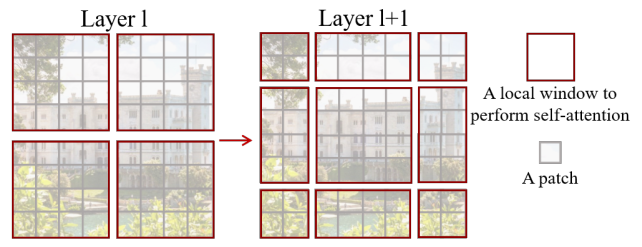
\includegraphics[width=\linewidth]{images/swint_transformer_patches.png}}
    \end{floatrow}
\end{figure}

\section{Detection models}

\subsection{Faster-RCNN}
TODO

\subsection{RetinaNet}
TODO

\subsection{YOLO family}
TODO

\subsection{EfficientDet}
EfficientDet tries to achieve a similar goal as EfficientNet: Propose a computationally effective architecture for object detection that would be scalable. Since efficient backbone architecture was alrady proposed \cite{Tan2019a}, they focus mainly on featue fussion from multiple layers. Based on the study of FPN, PANet, and NAS-FPN Bidirectional feature pyramid network (BiFPN) was proposed as the most computationally effective neck architecture \cite{Tan2019}; it consists of multiple BiFPN blocks stacked on top of each other, see \ref{fig:necks}. The count of those blocks is dependent on the size of the used backbone.

\subsection{Models for image segmentation}
\subsubsection{U-Net}
\begin{figure}
    \centering
    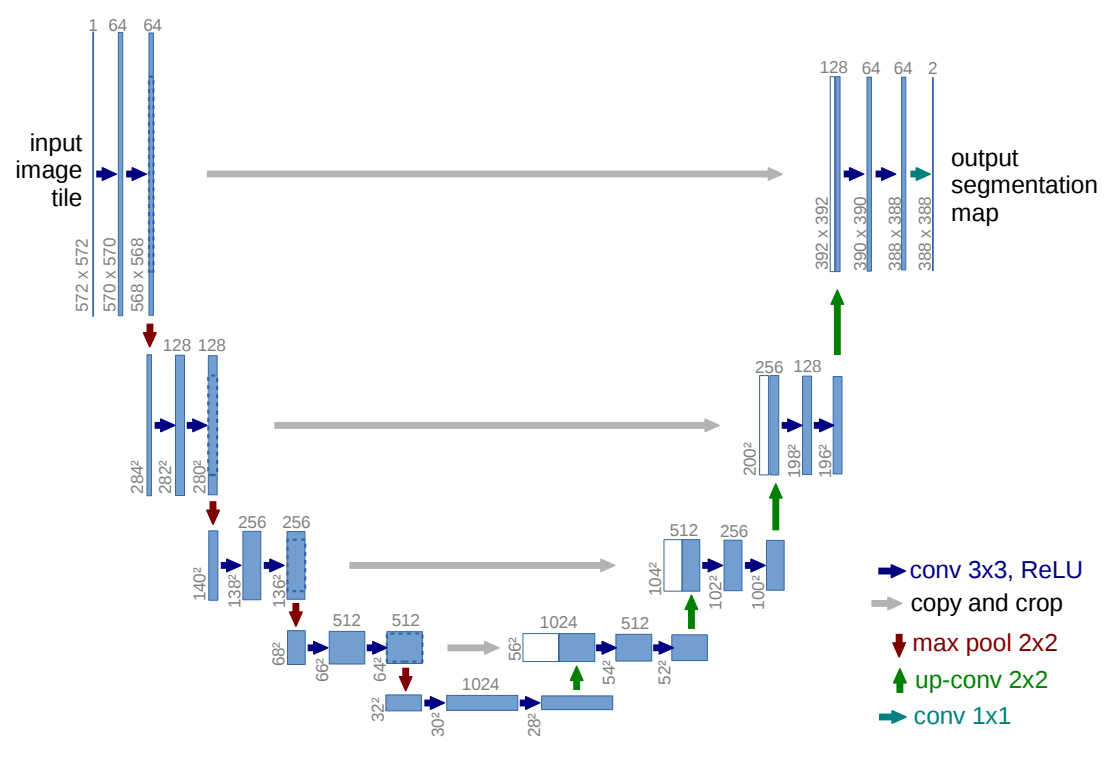
\includegraphics[width=\linewidth]{images/U-Net.png}
    \caption{Architecture of U-Net model, source \cite{Ronneberger2015}}
    \label{fig:unet_architecture}
\end{figure}
U-Net is an architecture for semantic segmentation. It has an encoder-decoder structure as can be seen in figure \ref{fig:unet_architecture}. The decoder extracts feature maps from the input image with increasing semnatical stregth throught the layers. In the middle of the network is so called bottle-neck layer with the strongest semnatical information about the image, but lacking information about high-resolution details of the input image. Hence when the information from the bottle neck is decoded by the decoder, it is combined with information from shallower layer, which contains information about image details, required to obtain a precise dense prediction.
\newline
The decoder proposed by Rennenberger et al. \cite{Ronneberger2015} can be replaced by a general-purpose backbone, as demonstrated by Baheti et al. \cite{Baheti2020}, who used EfficientNet as the backbone.

\section{Model ensembling in object detection}

Let say we have $M$ different models, each of them predicting $\mathcal{B}_i = \left\{b_1,...,b_N \right\} $ bounding boxes and $\mathcal{S}_i = \left\{ s_1,...,s_N \right\} $ confidence values for a given image corresponding to a single class. We merge predictions of all models together, it is possible to use weights $\mathit{W} = \{w_1,...,w_M \}$ to express our prior belief in given model. Set of all boxes $\mathcal{B}$ and confidence scores $\mathcal{S}$ is thus obtained by:
\begin{align}
    \mathcal{B} = \bigcup_{i=1}^{M} B_i \quad, \mathcal{S} = \bigcup_{i=1}^{M} S_i * w_i / F,
\end{align}
where F is optional normalization constant. It's only purpose is to ensure, that confidence score will be less than 1 after the ensembling. Commonly used value for F is $\frac{1}{M} \sum_{i=1}^M w_i$. After obtaining sets $\mathcal{B}$ and $\mathcal{S}$ we post-process them by one of the following algorithms: Non-maximal supression, soft non-maximal supression, non-maximum weighted supression or weighted boxes fusion.

\subsubsection{Non-maximal supression (NMS)}
In non-maximal supression, we first sort all boxes $\mathcal{B}$ by their confidence $\mathcal{S}$ in descending order. We go thru the sorted set $\mathcal{B}$ and check if any other box b in $\mathcal{B}$ has an overlap greater than the predefined threshold $N_t$; in that case, remove box $b$ from $\mathcal{B}$. More details regarding the NMS algorithm are in the pseudocode, which is in figure \ref{alg:nms}.
\begin{figure}
    \centering
    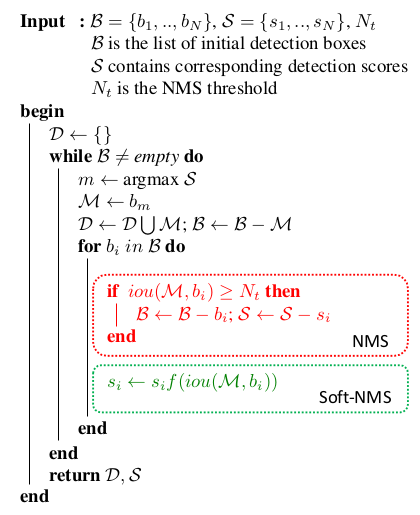
\includegraphics{images/nms_algo.png}
    \caption{Pseudo code of NMS and soft-NMS, source \cite{Bodla2017}}
    \label{alg:nms}
\end{figure}

\subsubsection{Soft non-maximal supression {Soft-NMS}}
Soft non-maximal supression extends the NMS algorithm by possibility to keep overlaping predictions if their confidences are high. Insted of removing boxes with overlap, we decrease their confidence value by the follwing Gaussian penalty function:
\begin{align}
    s_i = s_i e^{-\frac{\text{iou}\left( \mathcal{M}, b_i \right)^2}{\sigma}}, \forall b_i \notin \mathcal{D}
\end{align}
Where $\mathcal{M}$ is the currently processed bounding box and $\mathcal{D}$ is the set of already processed boxes. After processing all boxes, those with $s_i < T$ are removed, where $T$ is confidence cut-off threshold \cite{Bodla2017}.

\subsubsection{Non-maximum weighted superssion (NMW)}
Non-maximum weighted supression does not remove boxes in the case of overlap, but merges them togehter by following formula:
\begin{align}
    \mathcal{M} & = \frac{\sum_{i=1}^n \omega_i \times b_i}{\sum_{i=1}^n \omega_i} \\
    \omega_i    & = s_i \times \text{iou} \left( b_i, b_{ argmax_i s_i} \right)
\end{align}
where $\mathcal{M}$ is the merged bounding box, for which no confidence value is computed \cite{Zhou2017,Solovyev2019}.

\subsubsection{Weighted boxes fusion (WBF)}
Weighted boxes fusion is combining boxes similarly to NMW. The main difference is the iterative approach to the fusion, outputting confidence for the merged box, and awareness of a number of models, which contributed to the prediction.
The steps of WBF are as follows \cite{Solovyev2019}:
\begin{enumerate}
    \item Sort $\mathcal{B}$ by $\mathcal{S}$ as in NMS.
    \item Declare empty lists \boldmath{L} and \boldmath{F}, that would be used to store boxes clusters and merged box respectively
    \item Iterate thru $\mathcal{B}$ and if there is a box in \boldmath{F} for which $IOU > \mathbf{Threshold}$ add the box from $\mathcal{B}$ to list \boldmath{L} on position corresponding to position of the matched box in \boldmath{F}. If no match is found add it to the end of \boldmath{L}.
    \item Recalculate box coordinates $\mathcal{M}$ and confidence $c$ in the list \boldmath{F} on the position where box was added to \boldmath{L} by formulas \ref{eq:wbf1}.
    \item After processing all boxes from $\mathcal{B}$ adjust confidence scores by formula \ref{eq:wbf2}, where $T$ is number of contributing boxes and $M$ is number of models used for ensembling.
\end{enumerate}
\begin{align}
    \mathcal{M} & = \frac{\sum_{i=1}^n c_i \times b_i}{\sum_{i=1}^n c_i} ,\quad c=\frac{\sum_{i=1}^{T}c_i}{T} \label{eq:wbf1} \\
    c           & = c * \frac{T}{M} \label{eq:wbf2}
\end{align}
